%!TEX root = ../dissertation.tex
% this file is called up by thesis.tex
% content in this file will be fed into the main document

\graphicspath{{8-conclusions/figures/}}

\chapter{Conclusions and Final Remarks}
\label{ch:conclusions}

This thesis has presented a number of novel approaches demonstrating the effectiveness of deep generative models in automatic music transcription research.
In this chapter, we summarize our findings and discuss the future prospects of this line of research.

\section{Summary and Takeaways}


Through the experiments and analyses conducted in this thesis, we have answered the research questions raised in Section~\ref{ch:introduction}.\ref{sec:subproblems}.
We summarize our findings and discuss the takeaways from the thesis in the following paragraphs, by addressing each of the research questions raised in Section~\ref{ch:introduction}.\ref{sec:subproblems}.

\uline{Question 1: What kinds of deep models and representations can be used for effectively extracting pitch from audio?}
In Chapter~\ref{ch:monophonic} where a data-driven method for monophonic pitch estimation is proposed, we have found that a frame-wise convolutional computation predicting a time-frequency representation is an effective way to extract pitch information from audio.
This approach is succesfully employed in the subsequent chapters of this thesis, where we predicted Mel spectrograms for music synthesis (Chapter~\ref{ch:synthesis}), piano-roll representation for music transcription (Chapter~\ref{ch:adversarial}), and both (Chapter~\ref{ch:timbre}).

\uline{Question 2: How does the choice of datasets affect the accuracy and the generalizability of a trained model?}
We have learned that the choice of dataset can cause a drastic effect in a transcription model's performance, and caution regarding the generalizability is needed when releasing a model as open-source.
For an open-source release of a pre-traind model, the best practice is to train the model using many datasets from various sources that are as diverse as possible, because audios in a single dataset are likely to be highly correlated, compared to image datasets~\cite{thickstun2018invariances}.
In general, the performance of a model is a function of the quality and the quantity of the dataset, very much more so than it is a function of the novelty in the model's design, and it is a motivating factor to develop automated data augmentation methods to be discussed in the next section.


\uline{Question 3: How can we encode the concept of timbre in a way that is useful for music synthesis and transcription?}
In Chapter~\ref{ch:synthesis}, we have presented a WaveNet-based music synthesis method that can learn a continuous timbre embedding space, on which one can interpolate between different timbres.
This is achieved by conditioning a recurrent neural network with the timbre embedding to produce instrument-specific Mel spectrograms.
The timbre embedding space encodes continuous variations in musical timbre in which it is possible to interpolate timbres between points, and it can contain the timbre of virtually unlimited number of instruments.
How to reduce discontinuities and irregularities to make smoother timbre transitions remains a future work.

\uline{Question 4: How can a transcription model make informed predictions incorporating the knowledge of a music language model?}
In Chapter~\ref{ch:adversarial}, we have used a conditional generative adversarial network model to impose a prior on music transcription, borrowing ideas from image translation literature.
By appending an adversarial discriminator that encourages the resulting transcription to be realistic, this approach implements a music language model that works in conjunction with the Onsets and Frames transcription model.

\uline{Question 5: Can a music synthesizer component based on a deep generative model be used to improve music transcription?}
Lastly, in Chapter~\ref{ch:timbre}, we combined the ideas from the preceding chapters to create a music transcription model that can benefit from the musical knowledge contained in a music synthesizer model.
A synthesizer-aided transcription model achieves better recall than the equivalent model without a synthesizer, and it implies that the appended synthesizer provides useful information to the transcription model as a form of regularization.


The main takeaway from the approaches above is that it is crucial to find the best way to implement a good prior into a music transcription system, be it an adversarial discriminator or an appended music synthesis model.
Those priors can effectively serve as a regularizer to the problem and enable the model to be more efficiently trained with given amount of computing power and data.
This rule of thumb should be applied in future music transcription research; with the computing power and data availability becoming exponentially more abundant in the future, we can expect increased benefits of supplying the prior knowledge to task-specific models.


\section{Future Research Directions}

We discuss in this section how the automatic music transcription approaches proposed in this thesis can be extended and further improved in future research.
An immediate future research direction is to combine the findings of Chapter~\ref{ch:adversarial} and Chapter~\ref{ch:timbre} to create a music transcription system with both an adversarial discriminator and an appended synthesizer component.
Although left as out-of-scope in this thesis because of the computational constraints, this will in theory provide better regularization for the overall system and be able to achieve better performance in music transcription.


\begin{figure}
	\centering
	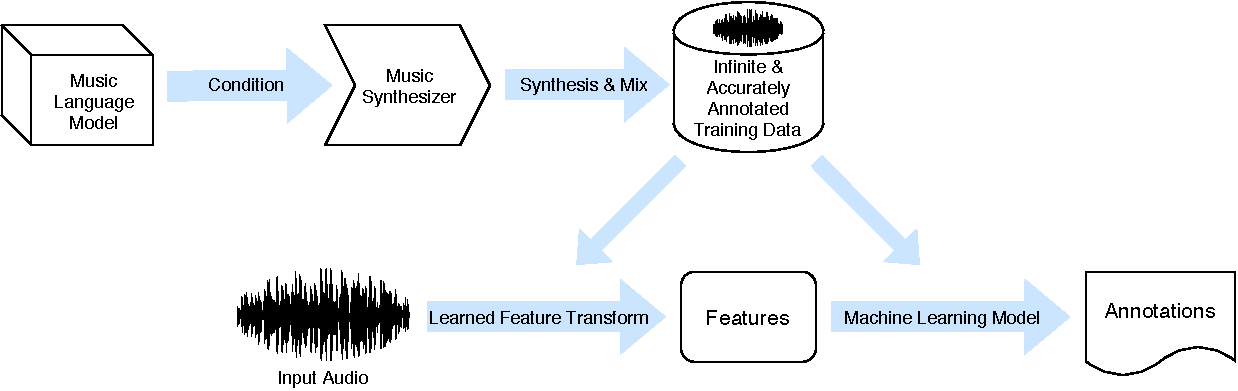
\includegraphics[width=\textwidth]{paradigms-5-proposed.pdf}
	\caption{A combination of music language model and music synthesizer can be used as an infinite source of accurately annotated training data for a transcription model.}\label{fig:unlimited-data}
\end{figure}

Data augmentation is a technique that can provide additional improvement in most music analysis tasks~\cite{mcfee2015muda}. % although it was not considered in the experiments in this thesis in order to keep the narratives focused on the novel approaches being introduced in each chapter.
While the conventional methods such as time stretch and pitch shift can be used for the purpose of music data augmentation, expressive music language models and music synthesis models can provide more powerful means of enriching the distribution of music data for training a transcription model.
This idea is illustrated in Figure~\ref{fig:unlimited-data}; an unlimited source of training data can be created using a combination of a powerful music language model and a good music synthesizer, which can then be used to train music analysis models such as a music transcription model.
When this pipeline can be successfully implemented, it is possible to scale the downstream model capacity and therefore improve the state-of-the-art performance in its analysis task, since the dataset size has been the main limitation in the recent data-driven music analysis models.
This idea is particularly promising considering the incredible performance of the recent transformer-based language models~\cite{vaswani2017attention} and generative pre-training approaches based on them~\cite{radford2018gpt,devlin2018bert}, which have been shown to be also effective in producing coherent symbolic music \cite{huang2019transformer}.

More powerful computational hardware will eventually enable a longer context length to be used in larger transformer models, which suggests another intriguing future research direction: to learn a music language model in the audio waveform domain.
This will help create a more expressive synthesizer component, which can be used to augmenting a music transcription model.
A compression method such as VQ-VAE~\cite{oord2017vqvae} would be helpful in allowing even longer context length to be used in such language model.

\begin{figure}[b!]
	\includegraphics[width=\textwidth]{turing.pdf}
	\caption{The \emph{transcriptional Turing test}, to test whether an automatic music transcription algorithm has reached human-level. When an automatically generated transcription is indistinguishable by an expert human listener from one produced by a skilled musician, it can be said that AMT is solved.}
	\label{fig:turing}
\end{figure}


Finally, in the discussion regarding the future of AMT, we need to consider the fundamental limitation on any music transcription task, either automatic or manual, and when it can be said that AMT is solved.
Polyphonic music contains a mixture of sounds with an indefinite number of notes being played simultaneously; even the most experienced musicians may not be able to identify every note.
It would be unreasonable to expect anyone to perfectly transcribe all notes in the score of an orchestral piece from an audio file, but it would be sensible for a trained musician to produce a version of the score that, when played by the same orchestra, sounds indistinguishable to the original recording.
Considering these limitations, passing this ``transcriptional Turing test'' as shown in Figure \ref{fig:turing}, rather than achieving 100\% accuracy on a certain dataset, should be the ultimate goal of automatic music transcription, at which point it could be said to mimic human expert-level knowledge on this task.

Considering the astounding progress of deep generative models in the domains such as image generation~\cite{karras2019stylegan} and natural language generation \cite{radford2018gpt}, it is reasonable to predict that generative modeling will play an important role in the coming decade for enabling a deeper computational understanding of music, to a degree that it becomes difficult to tell apart a machine-generated music transcription from one created by an expert musician.

